\chapter{Lambda Architecture}
\label{chap:lambda_architecture}

The Lambda architecture is a new solution for creating generic BigData systems \cite{MarzWarren201401}.
It provides model for scalable, fault-tolerant, distibuted processing of data.
It uses both batch and online processing to answer queries.
It provides human fault-tolerance, what is often overlooked in other approaches.
The Lambda architecture lets developer to concentrate on the logik and
algorithms, instead of thinking about maintainance of the system, e.g.
distributing computations, replication of dataset and how to manage intense grow of input data.

The core purpose of any information system is to answer specific queries having
data, gathered during functioning of the system.
Any query can be generically considered as a function of the whole dataset.
That means, that taking all available data, one can derive information, that
answers specific query.
[Running example]

Another important concept is that only raw data \mnote{raw data} must be
gathered in the system.
Its property is that it can not be derived from any other data.
It demands, nevertheless, that all types of queries, useful in the current
context, can be answered.
[Running example]

As a result of huge amounts of available data and its inherent rawness,
answering particular query is often unreasonably expensive or even infeasible. 
That is because query answer demands usually a piece of information, that is far
away from what raw data in the system describes.
It requires often execution of complex algorthims on the whole dataset.
In the BigData context that can mean hours of processing, while low-latency
response is typically a condition.
[Running example]

To solve this issue one can create batch views.
Batch view \mnote{batch view} is a specific data structure.
It contains derived data, that is a result of execution of specific algorithms
and aggregations on the whole dataset.
It is used for answering particular query.
Batch views are created in advance.
They can be used then in the query-time providing useful information.
[Running example]

Batch views are created in the infinite loop.
After the process of creation is completed, it starts again.
Processing all the data and creating batch views is high-latency operation.
It can take hours and even days to be done.
As a result batch views are always out-of-date.

To overcome this delay the Lambda architecture provides online processing.
It maintains additional data structures, called real-time views \mnote{real-time
view}.
They store information, derived from data arriving during current batch
processing.
Real-time views are normally different from batch views, and also more complex.
That is because they must be updated and available continuously, as new data
arrives.
This demands usage of such techniques like sketch algorithms.
It is described in all details in the particular chapter.
It worth to mention that real-time views contain often approximated information,
because of requirements they must obey.
But that is not a crucial problem, because they do not accumulate error for a
too long time.
Real-time view exists only during current batch processing.
When it is done, real-time views are dropped, and start to be created from the
beginning.

Summarizing, to answer the query system uses both things: batch views, computed
in the previous batch processing of the whole dataset, and real-time views,
gathering information from data coming during current batch processing.
Information from both types of views is then merged to provide answer to the
particular query.
Batch views provide information, that complete, but out-of-date for
several hours.
Real-time views contain information, gathered during current batch processing.

One key aspect of the Lambda architecture, that makes a difference with the
other approaches, is that human fault-tolerance is concerned inherently.
Human fault-tolerance \mnote{human fault-tolerance} is

This is important issue, because mistakes in programming code are guarantied.
And as a result, deleting or updating the data in a wrong way is also possible.

The Lambda architecture doesn't allow to modify data. This is called
immutability \mnote{immutability}.
Data can be only added, and never can be deleted or updated.
This leads to completely different model of storing data.
Instead of having simple tuple for a particular entity, every value of a tuple
is stored separately and has timestamp.
Such technique allows to have the whole history of editions of all attributes, what can be useful to make quesries that use history of changes.
At the same time the actual value is the one with the oldest timestamp.

\authorsection{General structure}{VI}

General view of the Lambda architecture is depicted on the
Figure~\ref{fig:lambda_architecture}.
It consists of three main elements: batch layer, serving layer and speed layer.
Batch layer contains master dataset, that allows only appending data.
One executes computations on the whole master dataset to obtain batch views,
that are useful to answer queries.
Serving layer is the place where batch views are stored.
It is also responsible for providing interface for making particular queries from those views.
Speed layer provides temporal views.
They contain sketches of data, that was obesrved during ongoing batch processing
in the batch layer.
It is important, because batch processing can last several hours or even longer.
Speed layer is much more complex than batch layer, and it provides only approximated results.
We discuss it in more details in the particular chapter.

\begin{figure}[H]
  \centering
  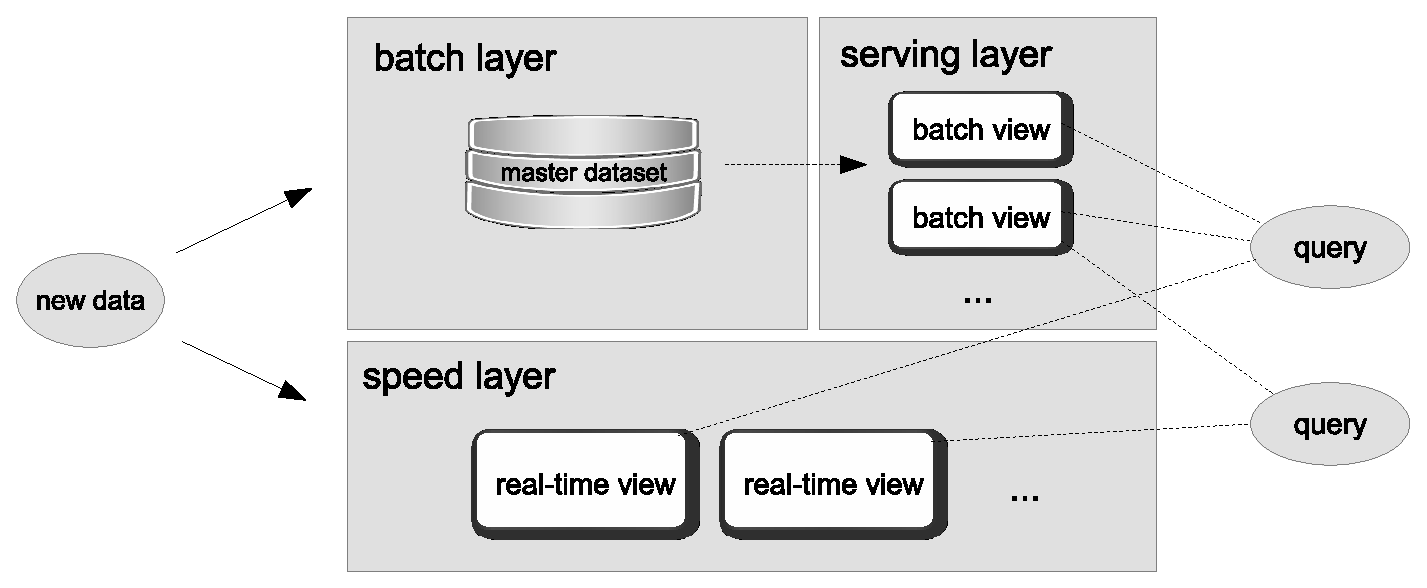
\includegraphics [width=0.9\textwidth]{images/LambdaArchitecture}
  \caption{General structure of the Lambda architecture}
  \label{fig:lambda_architecture}
\end{figure}

\authorsection{Batch layer}{VI}

Batch layer is the part of the Lambda architecture, that contains master dataset
and precomputes batch views, useful for answering queries.
One can think about master dataset as a very large list of records.
This is of course simplified representation, but for current discussion it is
enough.
When new piece of data arrives to the system, it is being added to the master dataset.
It can never change old records, or cause deletion.
This is what is called immutability of data.
This is a very important property, that provides human foult-tolerance, and at
the same time allows to execute queries on the whole history of changes.

Computation of batch views is being repeated continuously from scratch.
This is inherently distributed operation.
That means that developer doesn't have to think about concurrency and threads.
He only wrties simple one-threaded code, that is distributed than in the cluster.
MapReduce is a perfect example of a batch execution.
Apache Hadoop is an example of framework that can be used for computations in
the batch layer.

\authorsection{Serving layer}{VI}

Serving layer is a place where batch views are loaded and indexed for very fast
access.
It is represented by a specific distibuted database without ability to make random writes.
That simplifies things extremely, because opportunity to make random writes
brings most of complexity in databases.
One example of database that can be used for serving layer is ElephantDB.

\authorsection{Speed layer}{VI}

